{
\section{Convergence of the perturbed process}
\label{sec:proof-of-lem:resamplede-to-sampled}

\newcommand{\statenoweb}{S^{2D}_{\indepbm}}
\newcommand{\statewebapart}{S^{2D}_{\webnoargs}}
\newcommand{\statewebtogether}{S^{1D}_{\webnoargs}}
\newcommand{\twodim}{Y}

In this section we prove that
\statementoflemresampledetosampled{}.  This statement depends only on the
joint distribution of $\sampled$ and $\resamplede$.
We therefore define $\twodim^\epsilon = \twodim=(\resamplede, \sampled)$ (generally suppressing
the $\epsilon$ dependence in the notation). Let us describe the distribution of
$\twodim$
 as a two-dimensional random process.

We classify the behavior of the process into three states according to
the behavior of $\resamplede$ with respect to $\sampled$.
\begin{itemize}
\item If $\resamplede$ is in state $\statewebO$
and is coalesced with $\sampled$ we say $\twodim$ is in
state $\statewebtogether$.
\item If $\resamplede$ is in state $\statewebO$
and \emph{is not} coalesced with $\sampled$ we say $\twodim$ is in state $\statewebapart$.
\item If $\resamplede$ is in state $\statenowebO$
we say $\twodim$ is in state $\statenoweb$.
\end{itemize}
$\twodim$ starts
in $\statewebtogether$.  From $\statewebtogether$, $\twodim$
can only transition to $\statenoweb$.
This transition occurs when $\twodim$ hits the origin, as the coalesced
$\sampled$ and $\resamplede$ will continue together until they leave their
current half-plane.
From $\statenoweb$, $\twodim$ can only transition to
$\statewebapart$.  This transition occurs when $\resamplede$
leaves the $(-\epsilon,\epsilon)$
interval (i.e.\ $\twodim$ hits either of the $x=\pm\epsilon$ lines).
From
$\statewebapart$, $\twodim$ can either transition to $\statewebtogether$
if $\sampled$ and $\resamplede$ coalesce (i.e.\ $\twodim$ hits the line $x=y$)
or transition to $\statenoweb$ if $\resamplede$ hits $0$ (i.e.\ $\twodim$ hits
the $x=0$ line).
States and possible transitions of $\twodim$ are summarized in Figure
\ref{fig:twodimtranstab}.

The form of the labels given to the states is justified by the following.

\begin{observation*}
In $\statewebtogether$, $\twodim$ follows the law of a one-dimensional
Brownian motion.
In $\statewebapart$ and $\statenoweb$, $\twodim$ follows the law of a
two-dimensional Brownian motion.
\end{observation*}

Additionally observe that by the scale-invariance of Brownian motion,
the distribution of the sample paths of $\twodim^\epsilon/\epsilon$ is
independent of $\epsilon$.

\begin{figure}
\begin{center}
%  \begin{tabular}{c | l || c | c | c | c | }
\renewcommand{\arraystretch}{0.9}
\begin{tabular}{c|c|c|c|c|c|}
\cline{2-6}
 & State & Illustration & Law & Next & Trans. Cond. \\ \cline{1-6}
\multicolumn{1}{|c|}{\multirow{18}{*}{$\resamplede$}} &
\multicolumn{1}{|c|} {\multirow{6}{*}{$\statenoweb$}} &  & \multirow{6}{*}{indep.} & \multirow{6}{*}{$\statewebapart$} & \multirow{6}{*}{hits $\pm\epsilon$}     \\
\multicolumn{1}{|c|} {} & {} & {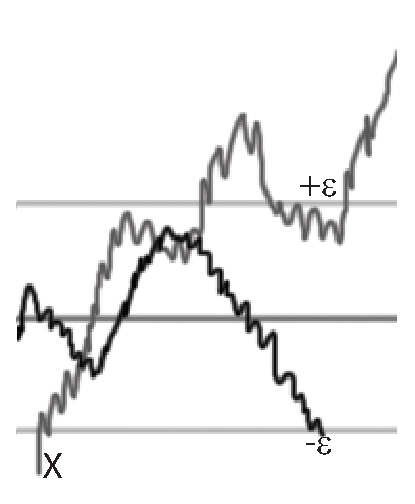
\includegraphics[scale=0.33]{r2dnc.eps}} & {} & {} &     \\ \cline{2-6}
\multicolumn{1}{|c|} {} &  \multirow{6}{*}{$\statewebapart$} &  & \multirow{6}{*}{indep.} & \multirow{3}{*}{$\statenoweb$} & \multirow{3}{*}{hits   $0$}\\
\multicolumn{1}{|c|} {} & {} & {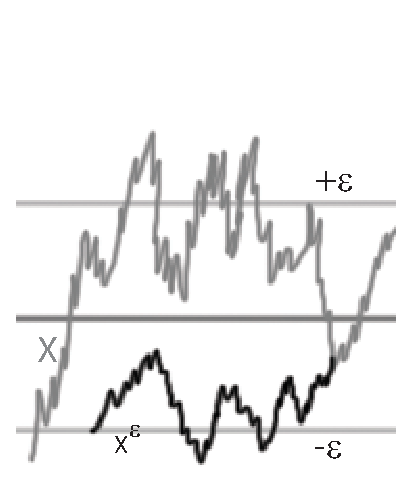
\includegraphics[scale=0.33]{r2dc.eps}} & {} & \multirow{-3}{*}{$\statewebtogether$} &   \multirow{-3}{*}{hits  $\sampled$}  \\ \cline{2-6}
\multicolumn{1}{|c|} {} & {\multirow{6}{*}{$\statewebtogether$}} & {}& \multirow{6}{*}{equal} & \multirow{6}{*}{$\statenoweb$} & \multirow{6}{*}{hits $0$}     \\
\multicolumn{1}{|c|} {} & {} & {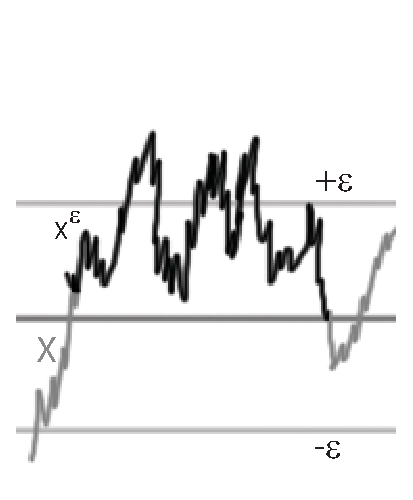
\includegraphics[scale=0.33]{r1d.eps}} & {} & {} &      \\ \hline\hline %\cline{1-6}
\multicolumn{1}{|c|}{\multirow{20}{*}{$\twodim=(x,y)$}} &
\multicolumn{1}{|c|} {\multirow{6}{*}{$\statenoweb$}} &  & \multirow{6}{*}{indep.} & \multirow{6}{*}{$\statewebapart$} & \multirow{6}{*}{$x=\pm\epsilon$}     \\
\multicolumn{1}{|c|} {\multirow{10}{*}{$x=\resamplede$}} & {} & {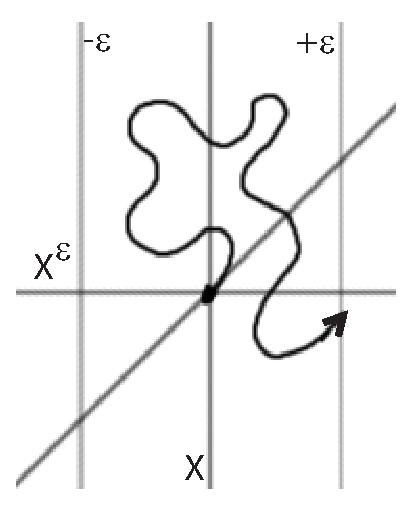
\includegraphics[scale=0.33]{s2dnc.eps}} & {} & {} &     \\ \cline{2-6}
\multicolumn{1}{|c|} {\multirow{10}{*}{$y=\sampled$}} &  \multirow{6}{*}{$\statewebapart$} &  & \multirow{6}{*}{indep.} & \multirow{3}{*}{$\statenoweb$} & \multirow{3}{*}{$x=0$}\\
\multicolumn{1}{|c|} {} & {} & {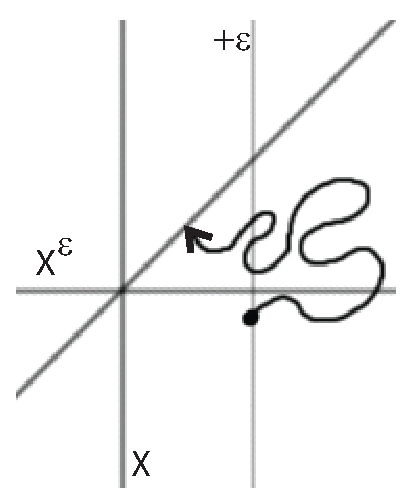
\includegraphics[scale=0.33]{s2dc.eps}} & {} & \multirow{-3}{*}{$\statewebtogether$} &   \multirow{-3}{*}{$x=y$}  \\ \cline{2-6}
\multicolumn{1}{|c|} {} & {\multirow{6}{*}{$\statewebtogether$}} & {}& \multirow{6}{*}{equal} & \multirow{6}{*}{$\statenoweb$} & \multirow{6}{*}{$x=y=0$}     \\
\multicolumn{1}{|c|} {} & {} & {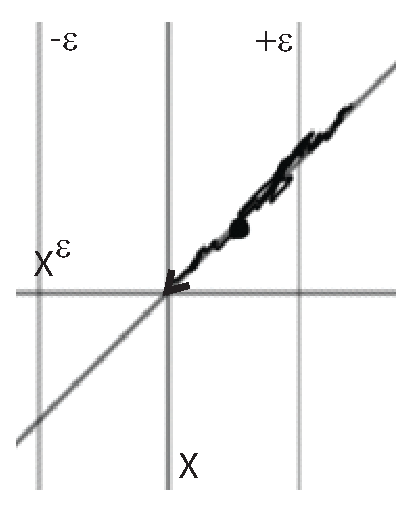
\includegraphics[scale=0.33]{s1d.eps}} & {} & {} &    \\
     \hline
  \end{tabular}
\end{center}
\caption{Illustrated states and transitions of $\twodim$}
\FIXME{}{Ohad to reorder rows to match order of state definitions}
\label{fig:twodimtranstab}
\end{figure}

\newcommand{\boundarylines}{A_\delta}

Define $\boundarylines=\{(x,y) \ :\  |x-y|=\delta \}$.
To prove Lemma \ref{lem:resamplede-to-sampled} we use the following
property of $\twodim$:

\newcommand{\farpoint}{(P,P)}
\newcommand{\probhitboundaryis}[1]{For given $P > 0$, $\delta > 0$ the probability that $\twodim$
  hits $\boundarylines$ before it hits $\farpoint$ is #1}

\begin{lemma}\label{lem:prob-hit-boundary-o1}
  \probhitboundaryis{$o(1)$ as $\epsilon \to 0$}.
\end{lemma}

We delay the proof of Lemma \ref{lem:prob-hit-boundary-o1} to Section
\ref{subsec:excursions-of-twodim}.

\begin{proof}[Proof of Lemma \ref{lem:resamplede-to-sampled}]

\TODO{}{We're implicitly assuming that the processes start at time $0$}
Lemma \ref{lem:resamplede-to-sampled} is equivalent to: for all $\delta > 0$, $u > 0$
\[
\P(\twodim_t \in \{(x,y) \ :\  |x-y|<\delta \} \text{ for all } t \in [0,u])\to1 \text{ as } \epsilon\to 0
\]
The above statement can be rephrased as

\vspace{12pt}
For all $\delta > 0$, $u > 0$,
the probability that before time $u$, $\twodim$ has hit $\boundarylines$
is $o(1)$ as $\epsilon \to 0$.
\TODO{}{Make this display better}
\vspace{12pt}

\RON{}{Probably need to choose choose $\epsilon_0$ such that for all
$\epsilon < \epsilon_0$ the probability that $\twodim$ hits $\boundarylines$ ...}
  We prove this as follows.  For any $\eta > 0$,
  choose $P$ so that the probability that standard Brownian motion
  travels from $0$ to $P$ in time less than $u$ is less than
  $\eta$.
  Apply Lemma \ref{lem:prob-hit-boundary-o1} to
  choose $\epsilon$ such that the probability that $\twodim$ hits
  $\boundarylines$ before $\farpoint$ is less than $\eta$.
  Then the probability that $\twodim$ hits $\boundarylines$ before $\farpoint$
  or takes less time than $1$ to reach $\farpoint$ is
  less than $2\eta$.
  Thus the probability that $\twodim$ hits $\boundarylines$ before
  time $1$ is less than $2\eta$.
\end{proof}

\subsection{Excursions of $\twodim$}
\label{subsec:excursions-of-twodim}

\TODO{}{This whole section perhaps needs reorganising}
In this section we prove the following, which is slightly stronger than
Lemma \ref{lem:prob-hit-boundary-o1}.

\newcommand{\loger}{\log 1/\epsilon}

\begin{lemma}\label{lem:prob-hit-boundary-o1loge}
  \probhitboundaryis{$O(\frac{1}{\loger})$}.
\end{lemma}

\newcommand{\origin}{(0,0)}

\newcommand{\excursionstart}{T}
  We begin by introducing the notion of an excursion of $\twodim$.
  Almost surely, the times at which $\twodim = \origin$ (which are stopping
  times) form an infinite discrete collection $\excursionstart_0 <
  \excursionstart_1 < \cdots$. We say ``the probability that an excursion
  hits a set $U$ is $p$'' if $\P(\twodim_t\in U \text{
  for some } t\in [\excursionstart_0, \excursionstart_{1}]) = p$.
  \FIXME{}{Provide a justification for the well-definedness of these
    stopping times, perhaps in terms of the states}

  Observe that by equidistribution this probability is the same when
  $t$ ranges over $[\excursionstart_i, \excursionstart_{i+1}]$, and
  note that the hitting events in question are independent.

\newcommand{\probexcursionhits}[1]{\P\left(\text{an excursion hits } #1\right)}

Our approach to proving Lemma \ref{lem:prob-hit-boundary-o1loge} is to
demonstrate that
\[
\probexcursionhits{\farpoint} \gg
\probexcursionhits{\boundarylines} \text { as } \epsilon \to 0
\]
This is
realized through the next couple of lemmas whose proofs we delay until Section
\ref{proofs-of-the-excursion-lemmas}.

\newcommand{\Omegaeloge}{\Omega(\epsilon\loger)}

\begin{lemma}
  \label{lem:Phitboundaryline}
  For given $\delta > 0$, $\probexcursionhits{\boundarylines}$ is $O(\epsilon)$.
\end{lemma}

\begin{lemma}
  \label{lem:Pabsorbedandtravelsfar}
  For given $P > 0$, $\probexcursionhits{\farpoint}$ is $\Omegaeloge$.
\end{lemma}

\newcommand{\Oe}{O(\epsilon)}

\begin{proof}[Proof of Lemma \ref{lem:prob-hit-boundary-o1loge}]
  $\twodim$ consists of a sequence of excursions, each of which satisfies
  exactly one of the following conditions
  \begin{itemize}
  \item the excursion hits $\boundarylines$ (with probability
    $O(\epsilon$))
  \item the excursion does not hit $\boundarylines$ but does hit
    $\farpoint$ (with probability $\Omegaeloge-\Oe$, which is itself
    $\Omegaeloge$)
  \item the excursion does not hit $\boundarylines$ or $\farpoint$
  \end{itemize}
  When $\twodim$ returns to $\origin$ a new excursion begins, which is independent of
  the previous excursions.  Thus the probability that the first
  condition occurs before the second is exactly the probability of the
  first as fraction of the sum of their probabilities, that is
  \[
  \frac{\Oe}{\Omegaeloge + \Oe} = O\left(\frac{1}{\loger}\right)
  \]
\end{proof}

\subsection{Proofs of the excursion lemmas}
\label{proofs-of-the-excursion-lemmas}
\newcommand{\tdh}{\rotproc^1}
\newcommand{\tdv}{\rotproc^2}
\newcommand{\rotproc}{Z}

\TODO{}{Perhaps should introduce more consistency between $\rotproc$
  and $\twodim$ in this proof}
{
\newcommand{\x}{\resamplede}
\newcommand{\y}{\sampled}
In this section we give the proof of Lemmas \ref{lem:Phitboundaryline} and
\ref{lem:Pabsorbedandtravelsfar}. For convenience we rotate (and scale)
$\twodim=(\x,\y)$, defining
\[\rotproc^\epsilon = \rotproc=(\tdh,\tdv)=\frac{1}{2}(\x+\y,\x-\y)\]

As for $\twodim$, $\rotproc$ has the following ``scale invariance''
property: the distribution of sample paths of $\rotproc^\epsilon /
\epsilon$ is independent of $\epsilon$.

\begin{proof}[Proof of Lemma \ref{lem:Phitboundaryline}]
Consider the process $\twodim$ between times $\excursionstart_0$ and
$\excursionstart_1$. Our goal is to show that with probability at least
$1-O(\epsilon)$, $\twodim$ arrives in $\statewebtogether$, before hitting
$\boundarylines$. That is because once it arrives at $\statewebtogether$ it
can never hit $\boundarylines$ before hitting $\origin$. Next, we observe the
following two auxiliary claims:

\begin{claim}\label{cl:tdv-together-estimate}
  Whenever $\tdv=0$ the probability that subsequently $\twodim$
  arrives at $\statewebtogether$ before $\tdv$ hits $\pm\epsilon/2$ is at
  least a constant (independent of $\epsilon$).
\end{claim}

\begin{claim}\label{cl:tdv-hitting-back-0-estimate}
  Whenever $\tdv=\pm\epsilon/2$ then there is probability equal to
  $\epsilon/\delta$ of $\tdv$ hitting $\pm\delta/2$ before it hits $0$.
\end{claim}

Claim \ref{cl:tdv-together-estimate} follows from scale invariance, while
Claim \ref{cl:tdv-hitting-back-0-estimate} is a standard martingale result on
Brownian motion (observing that on the relevant time interval $\tdv$ is a
standard Brownian motion).

The reduction of Lemma \ref{lem:Phitboundaryline} to those two claims is
similar to the proof of Lemma \ref{lem:prob-hit-boundary-o1loge}. Claims
\ref{cl:tdv-together-estimate} and \ref{cl:tdv-hitting-back-0-estimate} imply
that between two consecutive times when $\tdv=0$ which are separated
by times at which $\tdv = \pm\epsilon/2$,
\[
\frac{\P(\twodim\text{ hits }\boundarylines)}{\P(\twodim\text{arrives at }\statewebtogether)}
\le \frac{(1-C)(\epsilon/\delta)}{C} =O(\epsilon)
\]
\TODO{}{these probabilities are a bit confusing}
where $C$ is the constant of Claim \ref{cl:tdv-together-estimate}. As the
behavior of $\twodim$ is independent on those intervals, we deduce Lemma
\ref{lem:Phitboundaryline}.

\TODO{}{Why did we need independence?}
\end{proof}
}
\begin{proof}[Proof of Lemma \ref{lem:Pabsorbedandtravelsfar}]
\newcommand{\rotfarpoint}{(P,0)}
\newcommand{\segment}{[\epsilon,1] \cross \{0\}}
We bound below the probability that an excursion hits $\farpoint$,
i.e.\ $\rotproc$ hits $\rotfarpoint$ before returning to $\origin$.
We do this by considering the probability that the excursion takes
the following form: $\rotproc$ travels from $\origin$ to the line
segment $Q = [0, \epsilon] \cross \{\epsilon\}$, then hits the horizontal
axis for the first time in $\segment$, then travels to $\rotfarpoint$,
before returning to $\origin$.

After a stopping time at which $\twodim = \rotproc = \origin$ there is a positive probability $K$
that $\rotproc$ hits $Q$ before returning to $\origin$.
By scale invariance $K$ is independent of $\epsilon$.

Consider $\rotproc$ after hitting some point in $Q$.  We now
bound the hitting density of this process on the horizontal
axis.  Regardless of the point in $Q$, this density for points on
$\segment$ is at least
\[
\frac{1}{\pi\epsilon} \frac{1}{1 + (x/\epsilon)^2} dx
\]
This follows directly from the classical result that the hitting density
on a line of the two-dimensional Brownian motion is a Cauchy distribution
(see for example Theorem 2.37 of \cite{mortens-peres}).

On hitting a point $(x,0)$ for $x \in [\epsilon, 1]$ the process
transitions from state $\statewebapart$ to state $\statewebtogether$.
When in state $\statewebtogether$, $\rotproc$ behaves as a
one-dimensional Brownian motion on the horizontal axis until it hits
$\origin$.
By the same martingale argument which justifies
Claim \ref{cl:tdv-hitting-back-0-estimate}, the
probability of subsequently hitting $\rotfarpoint$ before $\origin$ is $x/2P$.
Integrating this against the hitting density we get that the probability that
$\rotproc$ started from some point in $Q$ hits the horizontal axis in $\segment$
and then travels to $\rotfarpoint$ before returning
to $\origin$ is at least
\[
\frac{1}{\pi P} \int_{\epsilon}^{1} \frac{x/\epsilon}{1 + (x/\epsilon)^2}
\, dx
=
\frac{\epsilon}{2\pi P} \log\left(\frac{1 + (1/\epsilon)^2}{2}\right)
,\text{ which is }
\Omegaeloge
\]
\TODO{}{This now looks slightly odd}
\end{proof}
}
